\section{Техническая часть}

\begin{tabularx}{\textwidth}{L{43mm}Y}
\toprule
\textbf{Компонент} & \textbf{Техническое решение} \\
\midrule
Платформа & Android 8.0+ (\code{minSdk 26}), Java; интерфейс для смартфонов и ТСД. \\
Сканирование & ML Kit Barcode Scanning, bundled-вариант, работа без сети. \\
Архитектура & Экран операции $\longleftrightarrow$ бизнес-операция $\longleftrightarrow$ адаптеры сканера и источника данных. \\
Совместимость & Адаптер ML Kit можно заменить на Zebra DataWedge, SDK ТСД или другую реализацию без изменения бизнес-логики. \\
Данные & Справочник товаров, ячейки и задания импортируются из подготовленных файлов. Операционные данные и результаты хранятся только на устройстве. \\
Документы & Фотография подписанной накладной сохраняется в отчёте о приёмке и доступна при его просмотре. \\
\bottomrule
\end{tabularx}

Сканирование возвращает код или ошибку и не изменяет результат операции до явного подтверждения сотрудником. Ошибки распознавания, неподходящий код и отсутствие доступа к камере отображаются понятным сообщением.

\clearpage
\subsection{Модель данных}

Ниже показана основная связь между сведениями о товаре и ячейками склада: \code{local\_inventory\_cache.cell\_id} ссылается на \code{storage\_cells.id}. Справочники, задания, результаты операций и отчёты о приёмке хранятся в локальной базе данных устройства.

\begin{figure}[htbp]
  \centering
  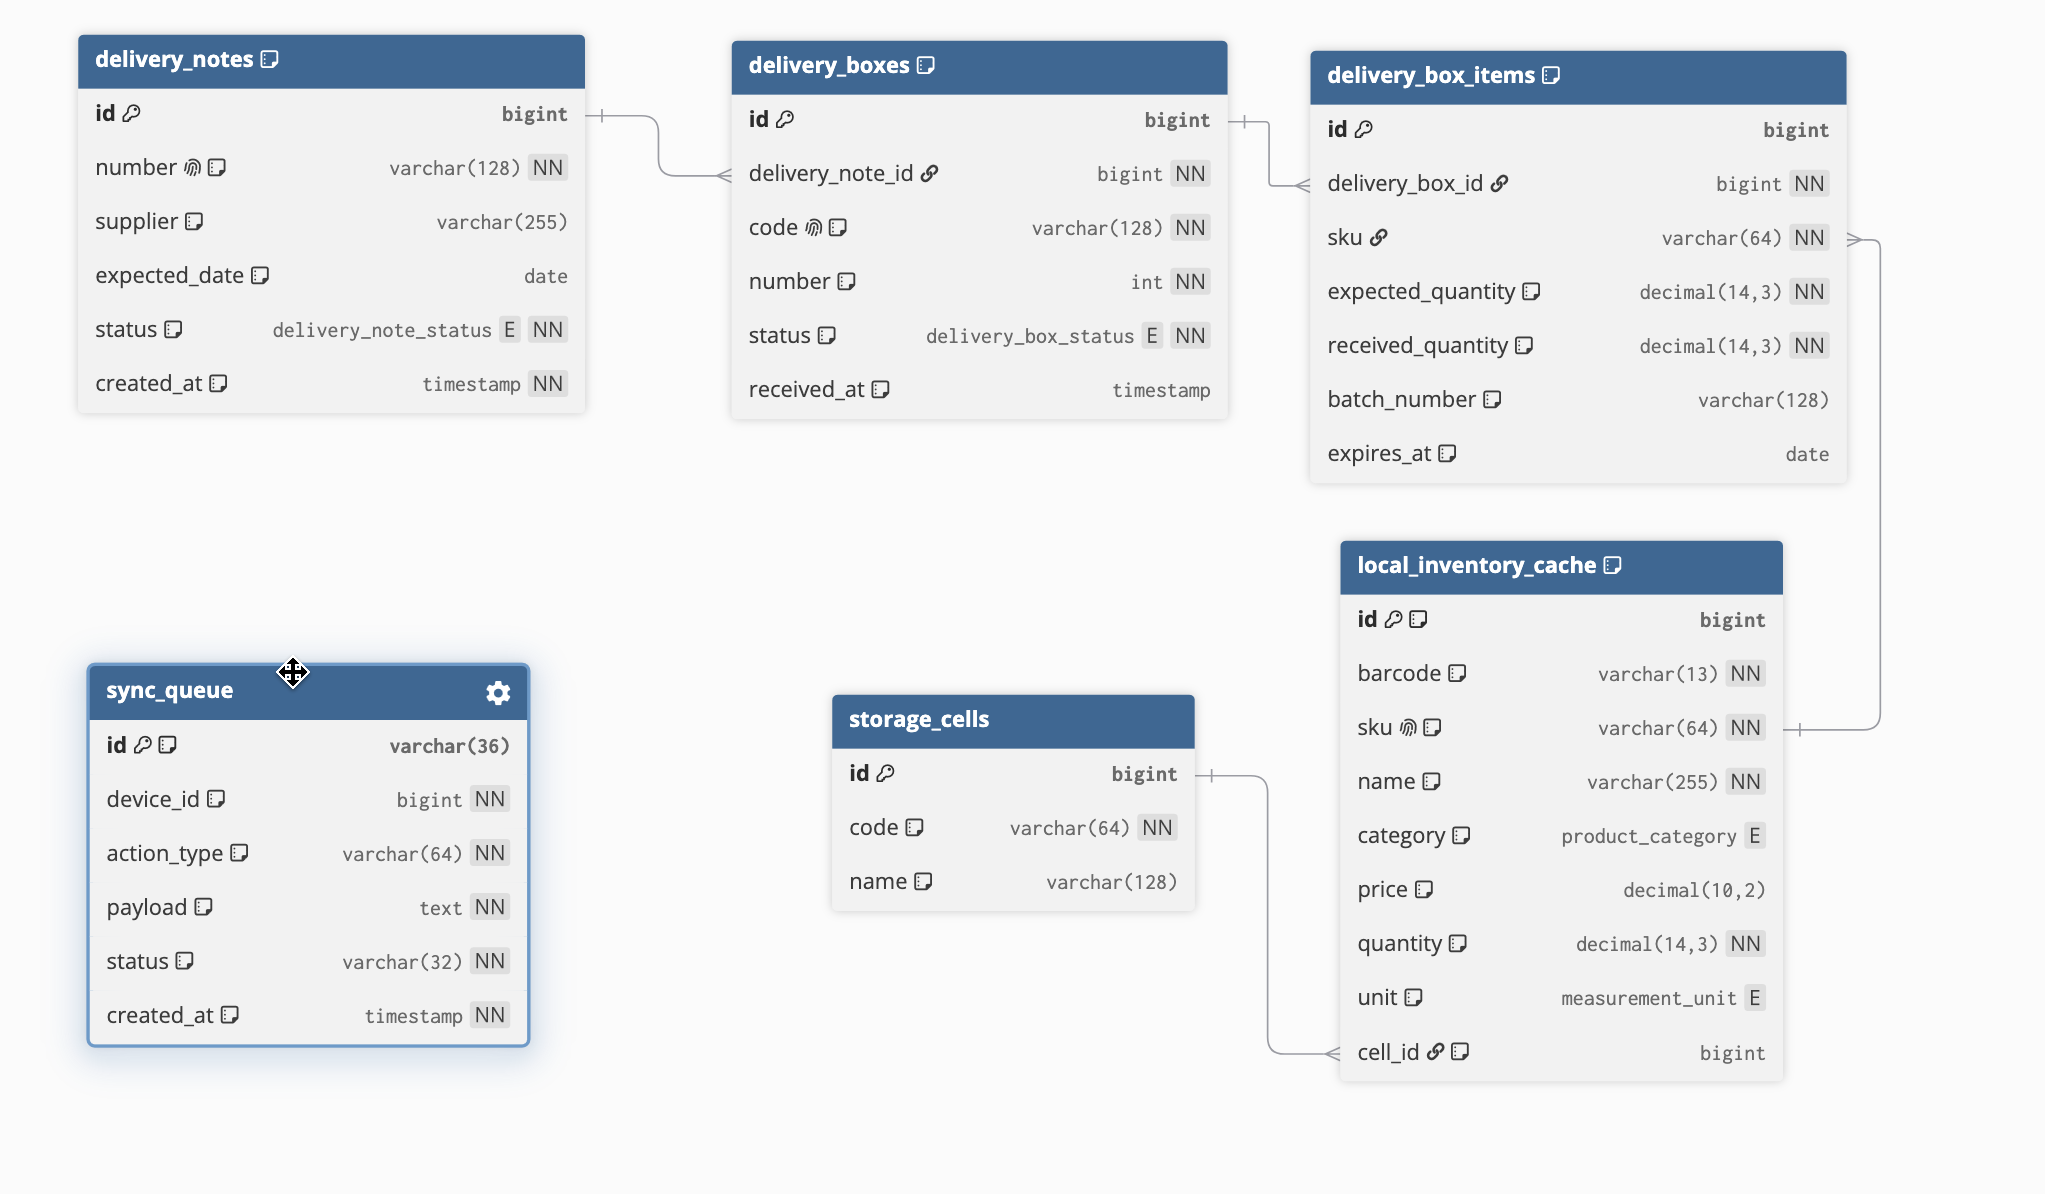
\includegraphics[width=0.90\textwidth]{assets/inventory-storage-er-diagram.png}
  \caption{Связь данных о товаре с ячейками склада}
  \label{fig:inventory-storage-er}
\end{figure}
